\documentclass[fleqn]{jbook}
\usepackage{physpub}

\begin{document}

\begin{question}{専攻 問題5}{}

\begin{subquestions}

\SubQuestion
金属の内部に電場$\vec{E}$が存在すると、$\vec{i} = \sigma \vec{E}$
に従う電流密度$\vec{i}$が生じる。ここで$\sigma $は導電率である。
しかし$\vec{E} = 0 $の場合にも、金属内部の温度$T$に勾配$\Grad T$
が存在すると電子は高温部から低温部へ流れ、そのとき生じる電流密度は、
$\vec{i_{th}}=\kappa \sigma \Grad T$と表される。この電流は熱電流、
係数$\kappa$は熱電能と呼ばれる。$\kappa$は金属の種類ごとに異なるが、
近似的には温度によらない定数とみなせる。以下の設問に答えよ。

\begin{subsubquestions}
\SubSubQuestion
1種類の金属導線の両端に温度差$\Delta T$を与えても、
持続的な電流は流れず、
その代わりにその両端に熱起電力と呼ばれる電位差$\Delta V$が発生する。
このときの$\Delta V$と$\Delta T$の関係を求めよ。また、
この熱起電力が発生する理由を、
電子の挙動を念頭において定性的に説明せよ。

\SubSubQuestion
種類のことなる金属(MとN)の導線を用いて図1のような閉回路を作り、
それらの金属の接合部$P_1$と$P_2$に温度差を与えると、
この閉回路には持続的な電流が発生する。その理由を定性的に説明せよ。

\end{subsubquestions}
\SubQuestion
図1のような閉回路は、熱電対と呼ばれ、
温度測定の素子として広く使われている。
この素子を使った温度の測定法について、以下の設問に答えよ。
\begin{subsubquestions}
\SubSubQuestion
図1の点Qに,図2で示す回路の端子Q1、Q2を挿入することで、
P1とP2の温度差を精度よく測定できる。ここでRは
抵抗値の大きな標準抵抗、VRは可変抵抗、Eは電池、Gは検流計、
Aは電流計である。いま、P1を試料に接触させた状態で、
VRを変化させて検流計を流れる電流をゼロに調整した。
このとき電流計にながれる電流の値から、
試料の温度とP2における温度との差が求められる。
この測定法の原理と利点を述べよ。ただし、
金属MとNの組み合わせに対して、
熱起電力と温度差との関係は既知とせよ。

\SubSubQuestion
いま、以上の方法で試料の絶対温度を求めたい。どうすればよいか、
要点を概念図に基づいて説明せよ。

\SubSubQuestion
こうして測定した試料の温度の正しさを左右する
と考えられる要因を列挙せよ。

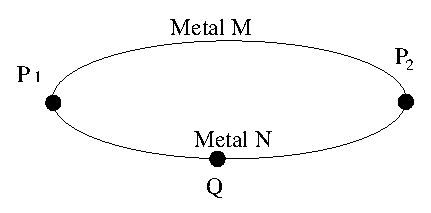
\includegraphics[clip,height=55mm,width=80mm]{1998phy5-1-1.eps}
\hspace{10mm}
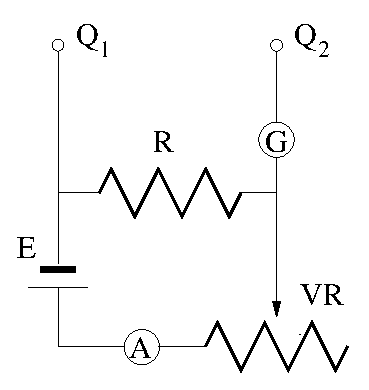
\includegraphics[clip,height=55mm,width=50mm]{1998phy5-1-2.eps}
\\
\hspace{25mm}
図1:熱電対の概念図。
\hspace{30mm}
図2:熱起電力の測定系の回路図。
\end{subsubquestions}
\end{subquestions}
\end{question}
\begin{answer}{専攻 問題5}{}
\begin{subanswers}
\SubAnswer
\begin{subsubanswers}

\SubSubAnswer
 
\[
\vec{i}=\sigma \vec{E}+\kappa\sigma \Grad T
\]
より、電流が流れなくなったときに、導線には
\[
\vec{E}=-\kappa \Grad T
\]
の電場が生じていると考えて、
\[
 \Delta V=\int Edx=\int -\kappa \Grad T=\kappa\Delta T
\]
従って、
\[
 \Delta V=\kappa \Delta T
\]
 の熱起電力が生じる。\\
 次に熱起電力が発生する理由を、電子の挙動を考慮して説明する。\\
 温度勾配によって電子が高温側から低温側に流れるために電流が生じる。
 そのために電子が低温側に集まり、それらの電子による電場(高温
 $\rightarrow$低温)が生じる。この電場は電子を高温側に戻す方向
 にできるため、ある程度低温側に電子が行くと、それ以上低温側に
 電子が流れなくなる。そのときの電子密度差による電場で熱起電力
 が発生する。
\SubSubAnswer
 前問の議論から、金属が違えば熱起電力が異なることは明らかであ
 る。従って、2つの金属の熱起電力の電位差を打ち消すために定常
 電流が流れていなければならない。
\end{subsubanswers}
\SubAnswer

\begin{subsubanswers}
\SubSubAnswer

\begin{itemize}
\item 原理\\
      測定回路を書き直しておく。\\
\begin{center}
\leavevmode
%
 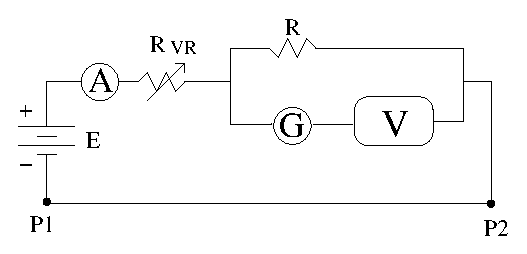
\includegraphics[clip]{1998phy5-1.eps}
\end{center}
\ \\
      図のVは金属導線M,Nによる熱起電力差である。熱起電力と温度との
      関係は既知であるからVが分かれば良い。いま、検流計に流れる電
      流が0になるように可変抵抗を調節すれば、電流計で電流iを計る
      ことでV=Riの関係より熱起電力差が求められる。
\item 利点\\
\begin{itemize}
\item 電流計の値を読むだけで測定が行えるので簡単かつ正確。(可変抵
      抗の値や、金属M,Nの抵抗値が分からなくても良い。)
\item 熱電対に電流が流れないので、熱電対にジュール熱が発生せず、試
      料の温度が変化しにくい。
\item 電流計を流れる電流をI、検流計を流れる電流をiとする。また、熱
      電対の金属Mの抵抗値を$r_M$、金属Nの抵抗値を$r_N$、測定したい
      熱電対の電位差を$V_{th}$とおくと、
\[
 V_{th}=R(i+I)+(r_M+r_N)i
\]
よりRが十分大きいので、
\[
 \left|\frac{r_M+r_N}{R}\right|\ll 1
\]
\[
 i\rightarrow i+\Delta i,\ I=0+\Delta I
\]
としたとき、
\[
 V_{th}\sim Ri+R(\Delta i+\Delta I)
\]
従って、誤差が評価しやすい。
\item Rが十分大きいので導線による電圧降下が無視できる。また、電流
      も小さくなるので回路で熱が発生しにくい。
\end{itemize}
\end{itemize}
\SubSubAnswer
 $T_1$を既知の温度にしておけば良い。(例えば水の3重点)

\SubSubAnswer
\begin{itemize}
\item 抵抗Rの精度
\item 検流計と電流計の精度
\item 試料と熱電対の断熱の具合い。(等温になっていなければならない。)
\end{itemize}

\end{subsubanswers}



\end{subanswers}
\end{answer}
\end{document}